\documentclass[10pt,a4paper]{article}
\usepackage[margin=2.0cm]{geometry}
\usepackage{microtype}
\usepackage{amsmath,amssymb}
\usepackage{booktabs,tabularx,array}
\usepackage{xcolor}
\usepackage{tikz}
\usetikzlibrary{arrows.meta,decorations.pathreplacing,patterns,positioning,calc,fit,backgrounds,shapes.geometric}
\usepackage{pgfplots}
\pgfplotsset{compat=1.17}
\usepackage{float}
\usepackage{caption}
\captionsetup{font=small,labelfont=bf}
\usepackage{enumitem}
\setlist{nosep,leftmargin=1.2em}
\usepackage[hidelinks]{hyperref}
\renewcommand{\arraystretch}{1.18}
\newcolumntype{L}{>{\raggedright\arraybackslash}X}
\newcommand{\opt}[1]{\texttt{-{}-#1}}

\definecolor{hone}{HTML}{2A78D6}   % haplotype 1
\definecolor{htwo}{HTML}{D35400}   % haplotype 2
\definecolor{art}{HTML}{C0392B}
\definecolor{nul}{HTML}{6C7A89}
\definecolor{ink}{HTML}{1B1B1B}
\definecolor{rep}{HTML}{EDA100}
\definecolor{fl}{HTML}{7F8C8D}
\definecolor{ok}{HTML}{1E8449}
\definecolor{pur}{HTML}{8E44AD}
\tikzset{
  arr/.style={-{Stealth[length=2.2mm]},thick,draw=ink!75},
  box/.style={draw=ink!70,rounded corners=2pt,fill=white,align=center,font=\small,inner sep=4pt},
  datb/.style={box,fill=nul!10},
  stp/.style={box,fill=hone!8},
  outb/.style={box,fill=ok!10},
  flank/.style={fill=fl!35,draw=fl!80},
  repeat/.style={fill=rep!55,draw=rep!90!black},
  ins/.style={fill=rep!90!black,draw=rep!60!black},
  snpA/.style={fill=hone,draw=hone!60!black,circle,inner sep=1.4pt},
  snpB/.style={fill=htwo,draw=htwo!60!black,circle,inner sep=1.4pt},
}
\def\fitPvarA{0.31}\def\fitPvarB{0.00}\def\fitPexpA{0.31}\def\fitPdll{135.3}\def\fitPLA{60}\def\fitPLB{69}
\def\fitNvarA{0.31}\def\fitNvarB{0.00}\def\fitNexpA{0.31}\def\fitNdll{138.9}\def\fitNLA{60}\def\fitNLB{69}

\def\curveYa{60}\def\curveYb{61}\def\curveYc{99}

\title{\textbf{tandemo}\\[2pt]\large True tandem-repeat length distributions per locus and haplotype\\
from PacBio HiFi reads: a learned read likelihood and a soft-phased mixture}
\author{Method document \quad\small(software version 0.1.0)}
\date{\small October 2026}

\begin{document}
\maketitle

\begin{abstract}
\noindent Observed read-length variation at a tandem repeat mixes sequencing noise with real variation between
molecules. \textbf{tandemo} separates the two in two stages. \emph{Network~1} learns, on a sample without repeat
instability, how a molecule of known length $L$ turns into an observed repeat length $Y$ in a HiFi read, given the
read's quality and the repeat's context: $p(Y\mid L,x)$. TRGT supplies the germline lengths, and HiPhase the phase
evidence. \emph{Stage~2} then estimates, for every locus and haplotype of a new subject, the distribution of
\emph{true} lengths $f_h(L)$: a point mass at the germline length plus a variable component. It integrates over
each read's unknown length and assigns reads to haplotypes softly, by het-SNV evidence along the whole read. The
output is one row per subject, locus and haplotype, ready for group comparison.
\end{abstract}

\tableofcontents
\bigskip

%=====================================================================
\section{Overview}

\begin{figure}[H]
\centering
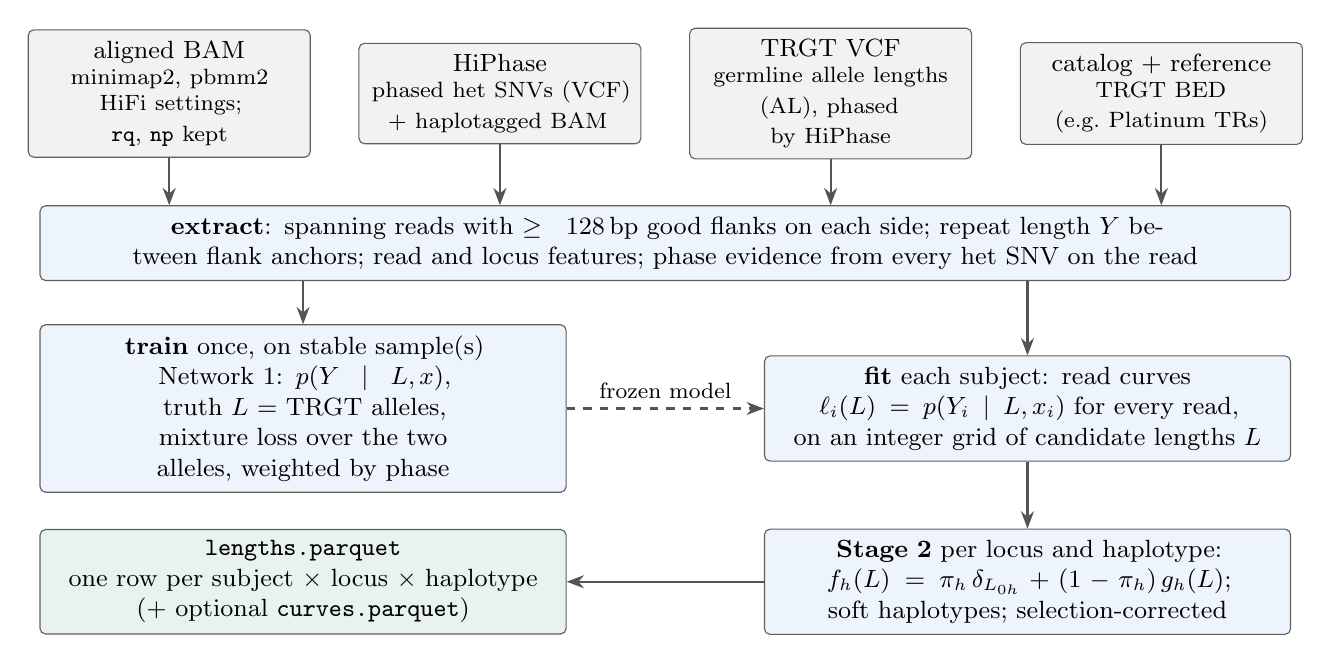
\begin{tikzpicture}[x=1cm,y=1cm]
\node[datb,text width=3.3cm] (bam) at (1.9,0) {aligned BAM\\\footnotesize minimap2, pbmm2 HiFi settings;\\\footnotesize \texttt{rq}, \texttt{np} kept};
\node[datb,text width=3.3cm] (hp) at (6.1,0) {HiPhase\\\footnotesize phased het SNVs (VCF)\\\footnotesize + haplotagged BAM};
\node[datb,text width=3.3cm] (trgt) at (10.3,0) {TRGT VCF\\\footnotesize germline allele lengths\\\footnotesize (AL), phased by HiPhase};
\node[datb,text width=3.3cm] (cat) at (14.5,0) {catalog + reference\\\footnotesize TRGT BED\\\footnotesize (e.g.\ Platinum TRs)};
\node[stp,text width=15.6cm] (ex) at (8.2,-1.9) {\textbf{extract}: spanning reads with $\geq128$\,bp good flanks on each side;
repeat length $Y$ between flank anchors; read and locus features; phase evidence from every het SNV on the read};
\foreach \n in {bam,hp,trgt,cat} {\draw[arr] (\n) -- (\n |- ex.north);}
\node[stp,text width=6.4cm] (tr) at (3.6,-4.0) {\textbf{train} once, on stable sample(s)\\
Network~1: $p(Y\mid L,x)$, truth $L$ = TRGT alleles,\\ mixture loss over the two alleles, weighted by phase};
\node[stp,text width=6.4cm] (cv) at (12.8,-4.0) {\textbf{fit} each subject: read curves\\
$\ell_i(L)=p(Y_i\mid L,x_i)$ for every read,\\ on an integer grid of candidate lengths $L$};
\draw[arr] (tr.north |- ex.south) -- (tr.north); \draw[arr] (cv.north |- ex.south) -- (cv.north);
\draw[arr,dashed] (tr) -- node[above,font=\footnotesize]{frozen model} (cv);
\node[stp,text width=6.4cm] (s2) at (12.8,-6.2) {\textbf{Stage~2} per locus and haplotype:\\
$f_h(L)=\pi_h\,\delta_{L_{0h}}+(1-\pi_h)\,g_h(L)$;\\ soft haplotypes; selection-corrected};
\draw[arr] (cv) -- (s2);
\node[outb,text width=6.4cm] (pq) at (3.6,-6.2) {\texttt{lengths.parquet}\\ one row per subject $\times$ locus $\times$ haplotype\\
(+ optional \texttt{curves.parquet})};
\draw[arr] (s2) -- (pq);
\end{tikzpicture}
\caption{The pipeline. Network~1 is trained once, on one or more stable samples, and then frozen. Every subject is
extracted and fitted on its own.}
\end{figure}

The central distinction (from the framework this implements) is between \emph{measurement} and \emph{biology}:
\begin{itemize}
\item \textbf{Measurement}, Network~1: if a molecule were $L$ bases long, how likely is each observed length $Y$ in
this read? This depends on the read and the repeat, never on the subject's biology.
\item \textbf{Biology}, Stage~2: how are true lengths distributed among the molecules of one haplotype? Each read's
own length is unknown and is summed out, never assigned.
\end{itemize}

%=====================================================================
\section{From aligned reads to observations}

\subsection{Which reads, and how $Y$ is measured}

\begin{figure}[H]
\centering
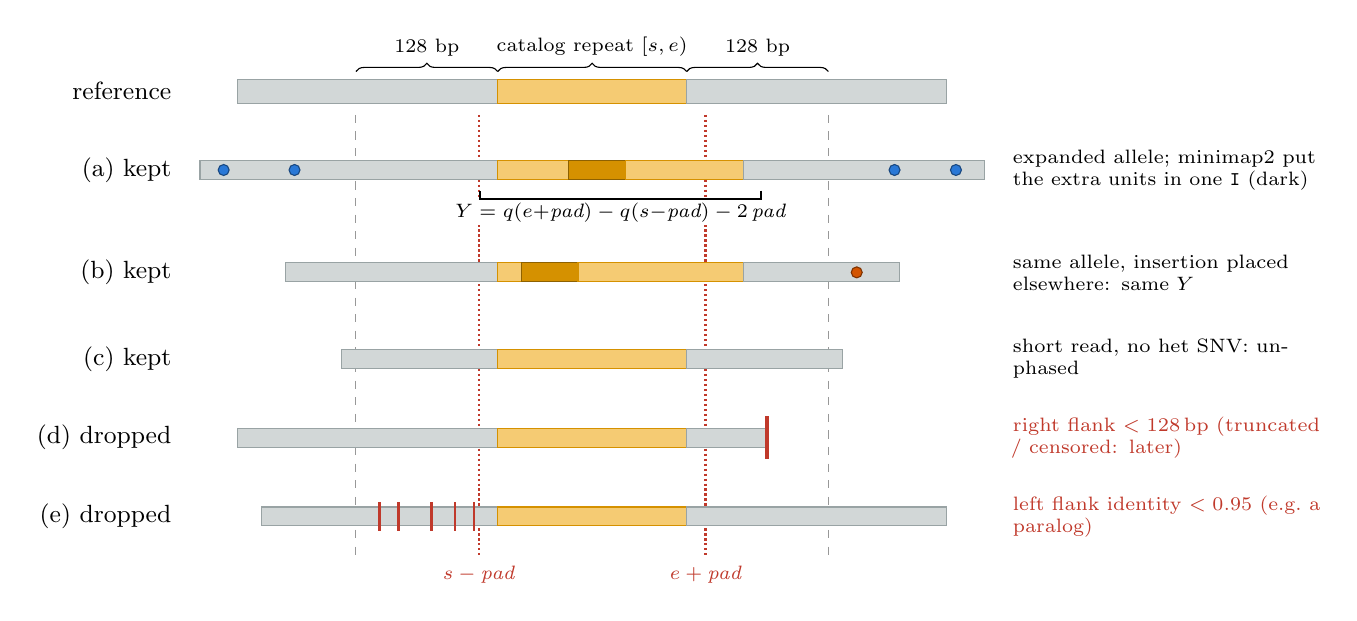
\begin{tikzpicture}[x=0.6mm,y=1mm]
\tikzset{note/.style={font=\scriptsize,anchor=west,text width=3.9cm,align=left}}
% reference
\node[anchor=east,font=\small] at (-12,60) {reference};
\fill[flank] (0,58.5) rectangle (55,61.5); \fill[repeat] (55,58.5) rectangle (95,61.5); \fill[flank] (95,58.5) rectangle (150,61.5);
\draw[decorate,decoration={brace,amplitude=3pt}] (55,62.5) -- node[above=2pt,font=\scriptsize]{catalog repeat $[s,e)$} (95,62.5);
\draw[decorate,decoration={brace,amplitude=3pt}] (25,62.5) -- node[above=2pt,font=\scriptsize]{128 bp} (55,62.5);
\draw[decorate,decoration={brace,amplitude=3pt}] (95,62.5) -- node[above=2pt,font=\scriptsize]{128 bp} (125,62.5);
\draw[dashed,ink!45] (25,57) -- (25,1); \draw[dashed,ink!45] (125,57) -- (125,1);
\draw[densely dotted,art,thick] (51,57) -- (51,1) node[below,font=\scriptsize,art]{$s-\textit{pad}$};
\draw[densely dotted,art,thick] (99,57) -- (99,1) node[below,font=\scriptsize,art]{$e+\textit{pad}$};
% (a)
\node[anchor=east,font=\small] at (-12,50) {(a) kept};
\fill[flank] (-8,48.8) rectangle (55,51.2); \fill[repeat] (55,48.8) rectangle (70,51.2);
\fill[ins] (70,48.8) rectangle (82,51.2); \fill[repeat] (82,48.8) rectangle (107,51.2); \fill[flank] (107,48.8) rectangle (158,51.2);
\foreach \x in {-3,12,139,152} {\node[snpA] at (\x,50) {};}
\draw[|-|,thick] (51,46.3) -- node[below,font=\scriptsize,fill=white,inner sep=1pt]{$Y=q(e{+}\textit{pad})-q(s{-}\textit{pad})-2\,\textit{pad}$} (111,46.3);
\node[note] at (162,50) {expanded allele; minimap2 put the extra units in one \texttt{I} (dark)};
% (b)
\node[anchor=east,font=\small] at (-12,37) {(b) kept};
\fill[flank] (10,35.8) rectangle (55,38.2); \fill[repeat] (55,35.8) rectangle (60,38.2);
\fill[ins] (60,35.8) rectangle (72,38.2); \fill[repeat] (72,35.8) rectangle (107,38.2); \fill[flank] (107,35.8) rectangle (140,38.2);
\node[snpB] at (131,37) {};
\node[note] at (162,37) {same allele, insertion placed elsewhere: same $Y$};
% (c)
\node[anchor=east,font=\small] at (-12,26) {(c) kept};
\fill[flank] (22,24.8) rectangle (55,27.2); \fill[repeat] (55,24.8) rectangle (95,27.2); \fill[flank] (95,24.8) rectangle (128,27.2);
\node[note] at (162,26) {short read, no het SNV: unphased};
% (d)
\node[anchor=east,font=\small] at (-12,16) {(d) dropped};
\fill[flank] (0,14.8) rectangle (55,17.2); \fill[repeat] (55,14.8) rectangle (95,17.2); \fill[flank] (95,14.8) rectangle (112,17.2);
\draw[art,very thick] (112,13.3) -- (112,18.7);
\node[note,art] at (162,16) {right flank $<128$\,bp (truncated / censored: later)};
% (e)
\node[anchor=east,font=\small] at (-12,6) {(e) dropped};
\fill[flank] (5,4.8) rectangle (55,7.2); \fill[repeat] (55,4.8) rectangle (95,7.2); \fill[flank] (95,4.8) rectangle (150,7.2);
\foreach \x in {30,34,41,46,50} {\draw[art,thick] (\x,4.2) -- (\x,7.8);}
\node[note,art] at (162,6) {left flank identity $<0.95$ (e.g.\ a paralog)};
\end{tikzpicture}
\caption{Reads at one locus. A read is kept when it covers 128 reference bases on \emph{each} side of the repeat,
with $\geq95\%$ alignment identity there and no clipping. $Y$ counts every read base between two anchors in the
unique flanks (default $\textit{pad}=10$), including bases minimap2 called insertions. Reads (a) and (b) come from
the same expanded allele: minimap2 placed the insertion at different points inside the repeat, but $Y$ is identical.
Coloured dots are phased het SNVs anywhere on the read (blue haplotype~1, orange haplotype~2).}
\label{fig:reads}
\end{figure}

\paragraph{Why measure between anchors?} Inside a repeat, minimap2's choice of where to place an indel is
arbitrary. Two reads of one allele can carry the extra units at different positions, and gap penalties sometimes
trade an indel for mismatches. The anchors sit outside the catalog interval (plus \textit{pad}) in unique flank
sequence. Every indel the aligner placed inside the repeat is therefore counted wherever it went, and repeat edges
that blur into partial units are measured consistently in every read.

\paragraph{Read filters.} Primary alignments only (no secondary, supplementary, duplicate or QC-fail records),
MAPQ $\geq20$, HiFi read quality $\texttt{rq}\geq0.99$. Truncated reads, which end inside the repeat, are not used
yet (Section~\ref{sec:later}).

\subsection{Phase evidence along the whole read}

\begin{figure}[H]
\centering
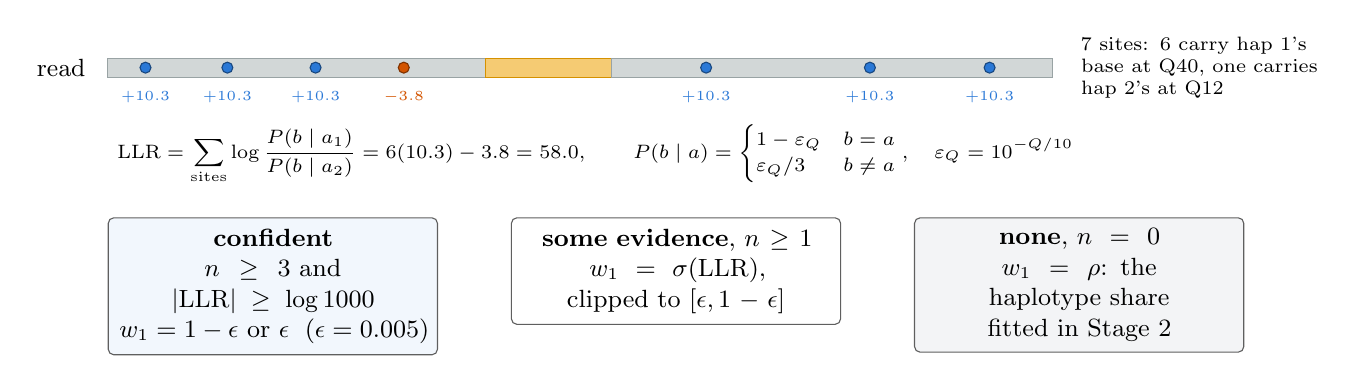
\begin{tikzpicture}[x=0.8mm,y=1mm]
\fill[flank] (0,30.8) rectangle (60,33.2); \fill[repeat] (60,30.8) rectangle (80,33.2); \fill[flank] (80,30.8) rectangle (150,33.2);
\node[anchor=east,font=\small] at (-2,32) {read};
\foreach \x in {6,19,33,95,121,140} {\node[snpA] at (\x,32) {}; \node[font=\tiny,hone] at (\x,28.3) {$+10.3$};}
\node[snpB] at (47,32) {}; \node[font=\tiny,htwo] at (47,28.3) {$-3.8$};
\node[font=\scriptsize,anchor=west,text width=3.2cm] at (153,32) {7 sites: 6 carry hap~1's base at Q40, one carries hap~2's at Q12};
\node[font=\scriptsize,anchor=west] at (0,21) {$\displaystyle
\mathrm{LLR}=\sum_{\text{sites}}\log\frac{P(b\mid a_1)}{P(b\mid a_2)}=6(10.3)-3.8=58.0,\qquad
P(b\mid a)=\begin{cases}1-\varepsilon_Q & b=a\\ \varepsilon_Q/3 & b\neq a\end{cases},\quad \varepsilon_Q=10^{-Q/10}$};
\node[box,anchor=north west,text width=3.9cm,fill=hone!6] at (0,13) {\textbf{confident}\\ $n\geq3$ and $|\mathrm{LLR}|\geq\log1000$\\
$w_1=1-\epsilon$ or $\epsilon$\; ($\epsilon=0.005$)};
\node[box,anchor=north west,text width=3.9cm] at (64,13) {\textbf{some evidence}, $n\geq1$\\
$w_1=\sigma(\mathrm{LLR})$,\\ clipped to $[\epsilon,1-\epsilon]$};
\node[box,anchor=north west,text width=3.9cm,fill=nul!8] at (128,13) {\textbf{none}, $n=0$\\
$w_1=\rho$: the haplotype share\\ fitted in Stage~2};
\end{tikzpicture}
\caption{Phase weight of a read. Every phased het SNV the read covers counts, not only those in the flanks. Only
sites in the locus's phase block (the PS of the phased TRGT record, or of the nearest het sites) count. Het indels
count too, when the read's bases from 10\,bp before to 10\,bp after the indel match one haplotype's sequence
exactly: they add $\pm\log\frac{1-e}{e}$ with $e=0.01$, or $e=0.05$ in a homopolymer run $\geq4$, where HiFi's
residual errors concentrate. Indels within 5\,bp of any catalog repeat are not used, since their alleles are repeat
lengths. $w_1$ is a \emph{prior} from germline
evidence alone. Length never enters it, so length cannot be used circularly to hide instability. The cap $\epsilon$
keeps one misphased read from forcing an outlier onto the wrong haplotype.}
\end{figure}

\subsection{Germline alleles from TRGT}
TRGT reports each allele's length over the catalog interval $[s,e)$ (\texttt{FORMAT/AL}). When HiPhase has phased
the TRGT VCF, allele~$k$ of the genotype belongs to haplotype~$k{+}1$ of that block. Otherwise, for training, the
orientation is taken from confidently phased reads: the orientation that puts each haplotype's median $Y$ nearer
its allele wins. Haploid calls (one AL value) give one haplotype.

\paragraph{Putting TRGT alleles on the scale of $Y$: the pads.} $Y$ spans more than the catalog interval: from
$s-\textit{pad}$ to $e+\textit{pad}$, minus the $2\,\textit{pad}$ anchor bases. The two pads are fixed 10\,bp
windows immediately outside the repeat, $[s-10,\,s)$ and $[e,\,e+10)$, with no further slop. A germline indel in
a pad changes every read's $Y$ but not TRGT's allele, so without a correction network~1 would learn it as a
systematic read error. Extraction therefore records, from the phased small-variant VCF, the net length change of
the germline indels in the two pads on each VCF haplotype ($d_1,d_2$), and training uses
\[
L_h = \mathrm{AL}_h + d_h,
\]
oriented to haplotypes with the same phase evidence as the alleles. Indels further from the repeat lie outside
$Y$ and do not matter. A locus is left out of training when its pads cannot be resolved:
\begin{center}\small
\begin{tabular}{@{}ll@{}}
\toprule
event & treatment \\
\midrule
indel inside a pad (homozygous, or het in the locus's phase block) & added to $L_h$ \\
insertion exactly at $s$ or $e$ (TRGT may or may not count it) & locus excluded (ambiguous) \\
deletion spanning $s$ or $e$ & locus excluded (ambiguous) \\
deletion crossing the outer pad edge $s-10$ or $e+10$ & locus excluded (ambiguous) \\
het pad indel unphased, or in another phase block & locus excluded (unphased) \\
\bottomrule
\end{tabular}
\end{center}
On HG002 chr4 (T2T, Platinum TRs), 1{,}446 of 503{,}547 genotyped loci (0.3\%) carry a pad indel; 8{,}859 are
excluded as ambiguous, mostly homopolymers and dinucleotides, and 91 as unphased.

%=====================================================================
\section{Network 1: the read-generation likelihood}

\subsection{What it outputs}

\begin{figure}[H]
\centering
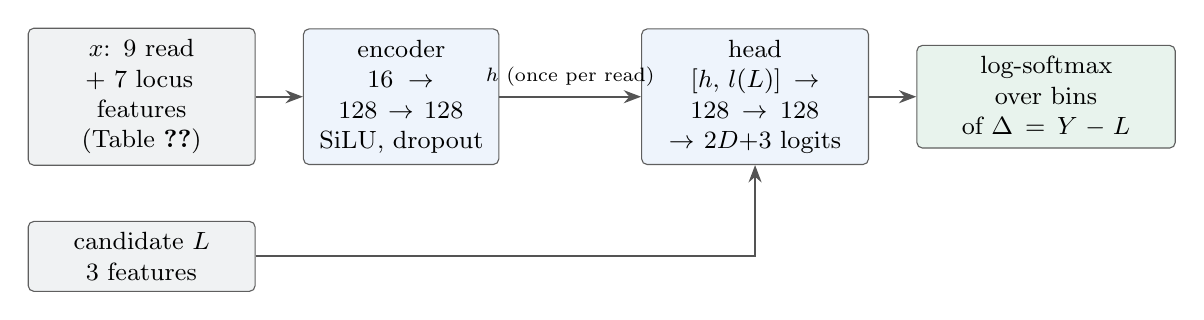
\begin{tikzpicture}[node distance=4mm and 6mm]
\node[datb,text width=2.6cm] (x) {$x$: 9 read + 7 locus\\features (Table~\ref{tab:features})};
\node[stp,right=of x,text width=2.2cm] (enc) {encoder\\ $16\to128\to128$\\ SiLU, dropout};
\node[datb,below=7mm of x,text width=2.6cm] (l) {candidate $L$\\ 3 features};
\node[stp,right=18mm of enc,text width=2.6cm] (head) {head\\ $[h,\,l(L)]\to128\to128$\\ $\to 2D{+}3$ logits};
\node[outb,right=of head,text width=3.0cm] (sm) {log-softmax over bins\\ of $\Delta=Y-L$};
\draw[arr] (x) -- (enc); \draw[arr] (enc) -- node[above,font=\scriptsize]{$h$ (once per read)} (head);
\draw[arr] (l) -| (head);
\draw[arr] (head) -- (sm);
\end{tikzpicture}

\vspace{3mm}
\begin{tikzpicture}
\begin{axis}[width=0.62\textwidth,height=4.2cm,ybar,bar width=4pt,ymode=log,log origin=infty,ymin=1e-7,ymax=1.5,
  xlabel={$\Delta=Y-L$ (bp)},ylabel={$p(\Delta\mid L,x)$},xmin=-11,xmax=11,
  xtick={-10,-5,-2,-1,0,1,2,5,10},tick label style={font=\scriptsize},label style={font=\small},
  extra x ticks={-11,11},extra x tick labels={tail,tail},extra x tick style={tick label style={font=\scriptsize,art}}]
\addplot[fill=hone!60,draw=hone] table[x=delta,y=p,col sep=comma] {figs/data/noise.csv};
\end{axis}
\end{tikzpicture}
\caption{Top: architecture. The encoder runs once per read, and the small head once per (read, candidate $L$). That
makes curves over hundreds of candidate lengths cheap. Bottom: the output for one read and one $L$ is a
distribution over the error bins: one bin per bp for $|\Delta|\leq D$ (default 50), plus a left and a right tail bin
whose mass is spread uniformly to $|\Delta|=T$ (5000). It sums to 1 over $Y$ for each $L$, so it is a proper
likelihood. It is \emph{not} normalised over $L$, and must not be.}
\label{fig:net}
\end{figure}

\paragraph{From outputs to a curve.} For read $i$, the network is evaluated at every candidate $L$ on the locus
grid, reading off the probability of the read's \emph{observed} $Y_i$:
$\ell_i(L)=p(Y_i\mid L,x_i)$. This curve is all Stage~2 sees of the read (Figure~\ref{fig:curves}).

\subsection{Features}
No feature encodes the read's own repeat length (no base counts or quality sums over the repeat), so the network
cannot read $Y$ off its input. The table is generated from \texttt{tandemo/features.py}.

\begin{table}[H]
\centering\small
\begin{tabularx}{\textwidth}{@{}l l l l L@{}}
\toprule
group & feature & source column & transform & meaning \\
\midrule
read & \texttt{rq\_phred} & \texttt{rq} & Phred & HiFi read quality as Phred, -10 log10(1 - rq), capped at 60 \\
read & \texttt{np\_log} & \texttt{np} & log(1+x) & CCS passes, log(1 + np) \\
read & \texttt{read\_len\_log} & \texttt{read\_len} & log10 & read length, log10 bp \\
read & \texttt{mapq} & \texttt{mapq} & x/60 & mapping quality / 60 \\
read & \texttt{has\_sa} & \texttt{n\_sa} & $x>0$ & read has supplementary alignments \\
read & \texttt{bq\_rep} & \texttt{bq\_rep} & x/40 & mean base quality over the read's repeat bases / 40 \\
read & \texttt{bq\_flank} & \texttt{bq\_flank} & x/40 & mean base quality over the two 128 bp flanks / 40 \\
read & \texttt{dist\_end\_log} & \texttt{dist\_end} & log(1+x) & bases from the repeat to the nearer read end, log \\
read & \texttt{flank\_err} & \texttt{flank\_id\_min} & 100(1-x) & error rate of the worse flank, 1 - identity, x100 \\
locus & \texttt{period\_log} & \texttt{period} & log2 & motif period, log2 bp \\
locus & \texttt{ref\_len\_log} & \texttt{ref\_len} & log(1+x) & reference repeat length, log bp \\
locus & \texttt{gc} & \texttt{gc} & x & GC fraction of the reference repeat \\
locus & \texttt{hp\_frac} & \texttt{hp\_frac} & x & fraction of repeat bases in homopolymer runs $\geq$ 4 \\
locus & \texttt{max\_hp\_log} & \texttt{max\_hp} & log(1+x) & longest homopolymer in the repeat, log \\
locus & \texttt{cx3} & \texttt{cx3} & x & 3-mer complexity of the repeat (distinct / possible) \\
locus & \texttt{flank\_cx} & \texttt{flank\_cx} & x & 3-mer complexity of the lower-complexity flank \\
candidate $L$ & \texttt{L\_log} & -- & -- & candidate true length, log(1 + L), standardised \\
candidate $L$ & \texttt{L\_vs\_ref} & -- & -- & log(1 + L) - log(1 + reference length): distance of the allele from the reference \\
candidate $L$ & \texttt{L\_units\_log} & -- & -- & log(1 + L / period): candidate length in motif units \\
\bottomrule
\end{tabularx}

\caption{Inputs of Network~1. Missing values (e.g.\ no \texttt{np} tag) are filled with the training median before
standardisation. The medians, means and standard deviations are stored in the model file.}
\label{tab:features}
\end{table}

\subsection{Training on a stable sample}
TRGT gives two allele lengths per locus. Which allele a training read came from is uncertain at heterozygous loci,
so reads are never hard-assigned:
\[
J=-\sum_i\log\big[\,w_{1i}\,p(Y_i\mid L_1,x_i)+(1-w_{1i})\,p(Y_i\mid L_2,x_i)\,\big],
\]
where $w_{1i}$ is the read's phase weight (0.5 without evidence). Homozygous loci reduce to one term.

\begin{figure}[H]
\centering
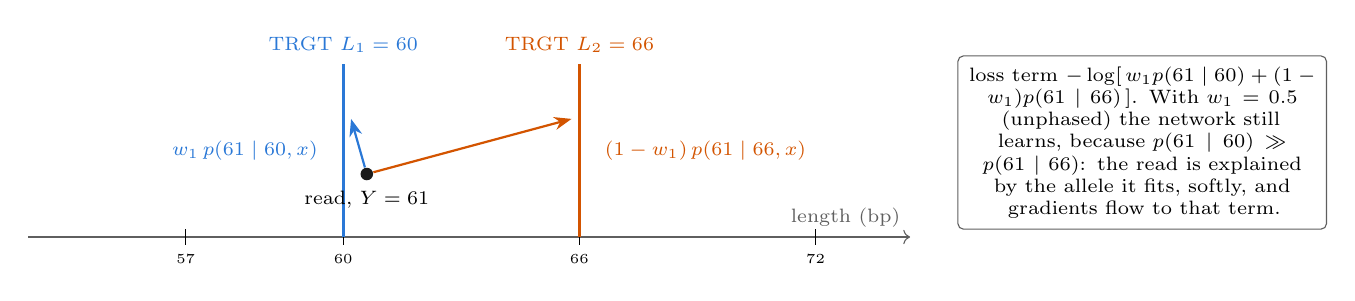
\begin{tikzpicture}[x=1mm,y=1mm]
\draw[->,ink!70] (0,0) -- (112,0) node[above left,font=\scriptsize]{length (bp)};
\foreach \x/\l in {20/57,40/60,70/66,100/72} {\draw (\x,-1) -- (\x,1); \node[font=\tiny,below] at (\x,-1) {\l};}
\draw[very thick,hone] (40,0) -- (40,22) node[above,font=\scriptsize]{TRGT $L_1=60$};
\draw[very thick,htwo] (70,0) -- (70,22) node[above,font=\scriptsize]{TRGT $L_2=66$};
\node[circle,fill=ink,inner sep=1.6pt,label={[font=\scriptsize]below:{read, $Y=61$}}] (y) at (43,8) {};
\draw[arr,hone] (y) -- (41,15);
\draw[arr,htwo] (y) -- (69,15);
\node[font=\scriptsize,hone,anchor=east] at (38,11) {$w_1\,p(61\mid60,x)$};
\node[font=\scriptsize,htwo,anchor=west] at (72,11) {$(1-w_1)\,p(61\mid66,x)$};
\node[box,anchor=west,text width=4.4cm,font=\scriptsize] at (118,12) {loss term $-\log[\,w_1 p(61\mid60)+(1-w_1)p(61\mid66)\,]$.
With $w_1=0.5$ (unphased) the network still learns, because $p(61\mid60)\gg p(61\mid66)$: the read is explained by
the allele it fits, softly, and gradients flow to that term.};
\end{tikzpicture}
\caption{One training read at a heterozygous locus. The two TRGT alleles are both candidates. The phase weight and
the network's own fit share the read between them, so no hard assignment is ever made.}
\end{figure}

\begin{table}[H]
\centering\small
\begin{tabularx}{\textwidth}{@{}l l L@{}}
\toprule
setting & default & why\\
\midrule
truth & TRGT \texttt{AL} & germline lengths of a sample without instability\\
loss & mixture NLL above & no hard allele assignment; uses heterozygous loci\\
validation & chr20--22 held out & reads of one locus never on both sides; else 10\% of loci by hash\\
optimiser & AdamW, lr $10^{-3}$, wd $10^{-5}$, batch 4096 & halve lr on plateau; early stop after 4 epochs\\
bins & $D=50$, $T=5000$ & HiFi errors are mostly $\pm1$--2\,bp; tails catch rare large errors\\
baseline & \texttt{-{}-empirical} & histogram per period $\times$ length class, same loss (EM); no read covariates\\
\bottomrule
\end{tabularx}
\caption{Network~1 training.}
\end{table}

\paragraph{Cautions.} TRGT's call is a consensus of the same reads, which pulls labels slightly toward them at low
depth; a second run of the sample for labels avoids this. Calibrate on samples whose chemistry and allele-length
range cover the subjects, since the network does not extrapolate far beyond its training lengths.

%=====================================================================
\section{Stage 2: the distribution of true lengths}

\subsection{Combining read curves}

\begin{figure}[H]
\centering
\begin{tikzpicture}
\begin{axis}[width=0.78\textwidth,height=4.6cm,xlabel={candidate true length $L$ (bp)},
  ylabel={$\ell_i(L)$ (scaled)},xmin=50,xmax=110,ymin=0,ymax=1.12,
  legend style={font=\scriptsize,at={(0.62,0.95)},anchor=north,draw=none,fill=white},
  tick label style={font=\scriptsize},label style={font=\small}]
\addplot[hone,thick,const plot mark mid] table[x=L,y=r0,col sep=comma] {figs/data/curves.csv};
\addlegendentry{read with $Y=\curveYa$}
\addplot[hone!50,thick,dashed,const plot mark mid] table[x=L,y=r1,col sep=comma] {figs/data/curves.csv};
\addlegendentry{read with $Y=\curveYb$}
\addplot[art,thick,const plot mark mid] table[x=L,y=r2,col sep=comma] {figs/data/curves.csv};
\addlegendentry{read with $Y=\curveYc$}
\end{axis}
\end{tikzpicture}
\caption{Three reads' likelihood curves from the noise model, scaled to peak 1. Each says which true lengths could
have produced the read. Multiplying the curves assumes all reads share one length; that is model M0. Stage~2
instead averages each curve over a distribution before multiplying across reads.}
\label{fig:curves}
\end{figure}

For haplotype $h$, the true-length distribution $f_h$ and the phase prior $a_{ih}$ give each read the marginal
likelihood
\[
p_i=\sum_h a_{ih}\;\frac{\sum_L \ell_i(L)\,f_h(L)\,s(L)}{\sum_L f_h(L)\,s(L)},\qquad
a_{ih}=\begin{cases}(w_{1i},\,1-w_{1i})&\text{het evidence}\\(\rho,\,1-\rho)&\text{none}\end{cases}
\]
The fit maximises $\sum_i\log p_i$ (computed with log-sum-exp) over the \emph{shape} of each $f_h$ and over $\rho$.
No read is ever given a single length. Which haplotype a read belongs to comes out as its posterior
\[
r_{ih}=a_{ih}\,\textstyle\sum_L\ell_i(L)f_h(L)s(L)/Z_h\;\big/\;p_i ,
\]
which combines the het prior with the length fit. An unphased read whose $Y$ sits at haplotype~2's $L_0$ lands
there without any het SNV.

\subsection{The model of $f_h$}

\begin{figure}[H]
\centering
\begin{tikzpicture}
\begin{axis}[name=a,width=0.52\textwidth,height=4.6cm,ybar,bar width=1.2pt,xmin=50,xmax=110,ymin=0,ymax=0.06,
  scaled y ticks=false,yticklabel style={/pgf/number format/fixed},
  xlabel={$L$ (bp)},ylabel={$f_h(L)$},title={\small parametric (default)},
  tick label style={font=\scriptsize},label style={font=\small}]
\addplot[fill=hone,draw=hone] table[x=L,y=f1,col sep=comma] {figs/data/f_parametric.csv};
\addplot[fill=htwo,draw=htwo] table[x=L,y=f2,col sep=comma] {figs/data/f_parametric.csv};
\draw[fill=art,fill opacity=0.12,draw=none] (axis cs:57.5,0) rectangle (axis cs:62.5,0.06);
\node[font=\tiny,art,anchor=north] at (axis cs:60,0.045) {no $g$};
\node[font=\tiny,hone,anchor=south west,fill=white,inner sep=1pt] at (axis cs:61,0.052) {$\uparrow\pi_1$};
\node[font=\tiny,htwo,anchor=south west,fill=white,inner sep=1pt] at (axis cs:70,0.052) {$\uparrow\pi_2$};
\end{axis}
\begin{axis}[at={(a.east)},anchor=west,xshift=10mm,width=0.52\textwidth,height=4.4cm,ybar,bar width=1.2pt,
  xmin=50,xmax=110,ymin=0,ymax=0.06,xlabel={$L$ (bp)},title={\small nonparametric (\opt{shape nonparametric})},
  scaled y ticks=false,
  tick label style={font=\scriptsize},label style={font=\small},yticklabels={}]
\addplot[fill=hone,draw=hone] table[x=L,y=f1,col sep=comma] {figs/data/f_nonparametric.csv};
\addplot[fill=htwo,draw=htwo] table[x=L,y=f2,col sep=comma] {figs/data/f_nonparametric.csv};
\end{axis}
\end{tikzpicture}
\caption{Fitted $f_h$ on a simulated locus: haplotype~1 (blue) with 30\% of molecules expanded around 84\,bp,
haplotype~2 (orange) stable at 69\,bp; 45 reads per haplotype, 30\% without phase evidence. Parametric fit:
$L_{01}=\fitPLA$, $1-\pi_1=\fitPvarA$ (truth 0.30), $1-\pi_2=\fitPvarB$, log-likelihood gain over M0
$=\fitPdll$. Nonparametric: $1-\pi_1=\fitNvarA$, $1-\pi_2=\fitNvarB$. The point masses (arrows) run off the top: the axis is cut at 0.06 to show $g$. The shaded band is the $g$ exclusion zone around $L_0$.}
\label{fig:fh}
\end{figure}

\[
f_h(L)=\pi_h\,\delta(L-L_{0h})+(1-\pi_h)\,g_h(L),\qquad g_h(L)=0\ \text{ for }|L-L_{0h}|<\Delta_g .
\]
\begin{itemize}
\item \textbf{Parametric} (default): $g_h$ is a skew-normal$(\xi,\omega,\alpha)$ evaluated on the integer grid and
renormalised, with $\omega\geq\omega_{\min}=\max(1,\text{period}/2)$. That is seven numbers per locus and haplotype,
stable at modest depth, and easy to compare across subjects.
\item \textbf{Nonparametric}: $g_h$ is a free distribution on the grid, fitted by EM with smoothing (EMS). Each
iteration computes expected counts over $L$, undoes the selection $s(L)$, smooths with a Gaussian kernel
(sd $\max(1,\text{period}/2)$), and restricts to the support. It finds bimodal or long-tailed shapes, at the price of
noisier estimates.
\item \textbf{Exclusion zone} $\Delta_g=\max(2,\text{period})$\,bp. Without it, a narrow $g$ sits on $L_0$ and
absorbs ordinary $\pm1$\,bp noise, making $\pi$ unidentifiable (Section~\ref{sec:checks}).
\end{itemize}

\subsection{Fitting}
\begin{enumerate}
\item \textbf{M0} ($\pi_h=1$): coordinate ascent over $(L_{01},L_{02})$ with $\rho$ by EM. It starts from the
phase-weighted modes, the TRGT alleles and the two largest pooled modes, each in both orders. The best is kept, so
haplotype labels follow the phase evidence.
\item \textbf{M1 parametric}: L-BFGS-B over $(\mathrm{logit}\,\pi_h,\ \xi_h,\ \log(\omega_h-\omega_{\min}),\ \alpha_h)$
and $\mathrm{logit}\,\rho$. It starts from shapes on both sides of $L_0$, a broad shape, and the most likely length
of each read M0 explains worst. Without those last starts, a single far-out read is never reached. Then a local
rescan of $L_0$ ($\pm2$ periods) and a polish.
\item \textbf{M1 nonparametric}: EMS from half a local bump and half a uniform floor over the support. EM cannot
grow mass where it starts at zero.
\item If M1 ends below M0 (it contains M0), M0 is reported.
\end{enumerate}

\subsection{Spanning selection}
\begin{figure}[H]
\centering
\begin{tikzpicture}
\begin{axis}[width=0.55\textwidth,height=3.8cm,xlabel={true length $L$ (bp)},ylabel={$s(L)$},ymin=0,ymax=1.05,
  scaled x ticks=false,xticklabel style={/pgf/number format/fixed,/pgf/number format/1000 sep={\,}},
  tick label style={font=\scriptsize},label style={font=\small}]
\addplot[pur,thick] table[x=L,y=s,col sep=comma] {figs/data/selection.csv};
\end{axis}
\end{tikzpicture}
\caption{A molecule is only observed when a read covers it plus 128\,bp on each side, so long molecules are
under-sampled. $s(L)\propto\sum_r\max(0,R_r-L-2\cdot128)$ over the lengths $R_r$ of all usable reads overlapping
the locus (here around 16\,kb). Stage~2 models the \emph{kept} reads as $f_h(L)s(L)$, so $f_h$ is the distribution
of molecules. \opt{no-selection} turns this off.}
\end{figure}

%=====================================================================
\section{Haplotypes and instability}

\begin{figure}[H]
\centering
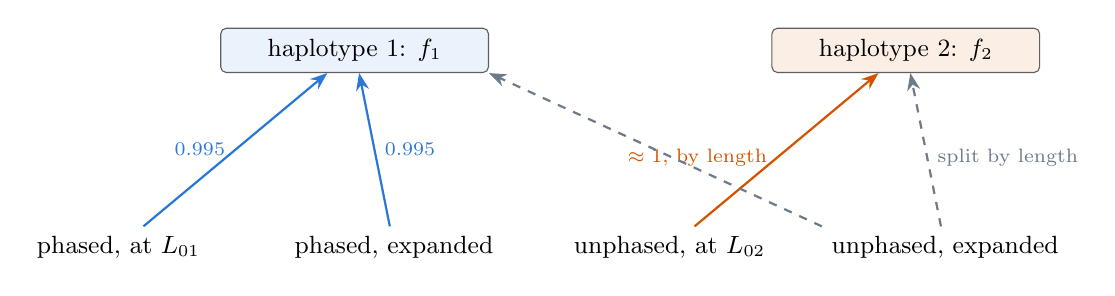
\begin{tikzpicture}[x=1mm,y=1mm]
\node[box,fill=hone!10,minimum width=34mm] (h1) at (35,30) {haplotype 1: $f_1$};
\node[box,fill=htwo!10,minimum width=34mm] (h2) at (105,30) {haplotype 2: $f_2$};
\node[font=\small] (ra) at (5,5) {phased, at $L_{01}$};
\node[font=\small] (rb) at (40,5) {phased, expanded};
\node[font=\small] (rc) at (75,5) {unphased, at $L_{02}$};
\node[font=\small] (rd) at (110,5) {unphased, expanded};
\draw[arr,hone] (ra) -- node[left,font=\scriptsize]{0.995} (h1);
\draw[arr,hone] (rb) -- node[right,font=\scriptsize]{0.995} (h1);
\draw[arr,htwo] (rc) -- node[left,font=\scriptsize,pos=0.45]{$\approx1$, by length} (h2);
\draw[arr,nul,dashed] (rd) -- node[right,font=\scriptsize,pos=0.45]{split by length} (h2);
\draw[arr,nul,dashed] (rd.north west) -- (h1.south east);
\end{tikzpicture}
\caption{A somatic expansion in a haplotype-1 molecule keeps haplotype~1's het SNVs, so phased reads carry it to
haplotype~1 only. Leakage between haplotypes happens only through reads without phase evidence, whose posterior is
decided by length. Leakage moves variable mass between haplotypes but never creates it.}
\end{figure}

\begin{table}[H]
\centering\small
\begin{tabularx}{\textwidth}{@{}l L@{}}
\toprule
column & meaning\\
\midrule
\texttt{L0}, \texttt{pi}, \texttt{var\_weight} & germline length; point-mass weight; $1-\pi$\\
\texttt{g\_xi}, \texttt{g\_omega}, \texttt{g\_alpha} & skew-normal parameters (parametric; NaN for nonparametric)\\
\texttt{g\_mean}, \texttt{g\_sd} & moments of $g$\\
\texttt{p\_exp}, \texttt{p\_con} & $P(L\geq L_0+\Delta)$, $P(L\leq L_0-\Delta)$ under $f_h$, $\Delta=\max(3,\text{period})$, fixed in advance\\
\texttt{mean\_abs\_dev} & $E|L-L_0|$ under $f_h$\\
\texttt{n\_eff}, \texttt{n\_phased\_eff} & reads received ($\sum_i r_{ih}$), of which with het evidence\\
\texttt{n\_var\_eff}, \texttt{n\_support} & expected reads from $g$; reads whose posterior favours $g$ ($>0.5$)\\
\texttt{unphased\_var\_frac} & share of the variable component carried by unphased reads (attribution confidence)\\
\texttt{pooled\_var\_weight}, \texttt{pooled\_p\_exp}, \texttt{pooled\_p\_con} & locus level, $\sum_h \text{share}_h\times\cdot$: unaffected by leakage\\
\texttt{share}, \texttt{rho} & haplotype share; fitted $\rho$\\
\texttt{ll\_m0}, \texttt{ll\_m1}, \texttt{d\_ll} & log-likelihoods and gain (evidence; no p-value)\\
\texttt{hap}, \texttt{hap\_rank} & HiPhase label (arbitrary per block); \texttt{short}/\texttt{long}/\texttt{tie}/\texttt{haploid} by $L_0$\\
\texttt{converged}, \texttt{at\_boundary}, \texttt{status} & fit diagnostics\\
\bottomrule
\end{tabularx}
\caption{\texttt{lengths.parquet}: one row per subject $\times$ locus $\times$ haplotype. The full $f_h$ can be rebuilt
from the parameters (parametric). \opt{write-curves} also stores every read's curve near its peak (within 20 log
units) with its phase weight, so Stage~2, or a group-level model, can be refitted without Network~1.}
\end{table}

\paragraph{Group comparison.} HiPhase labels are arbitrary per phase block, so haplotype~1 in one subject is
unrelated to haplotype~1 in another. Compare by \texttt{hap\_rank} (short/long allele), or use the pooled
columns. Read all subjects as one Parquet dataset (DuckDB, polars, pandas) and join a sample table.

\begin{figure}[H]
\centering
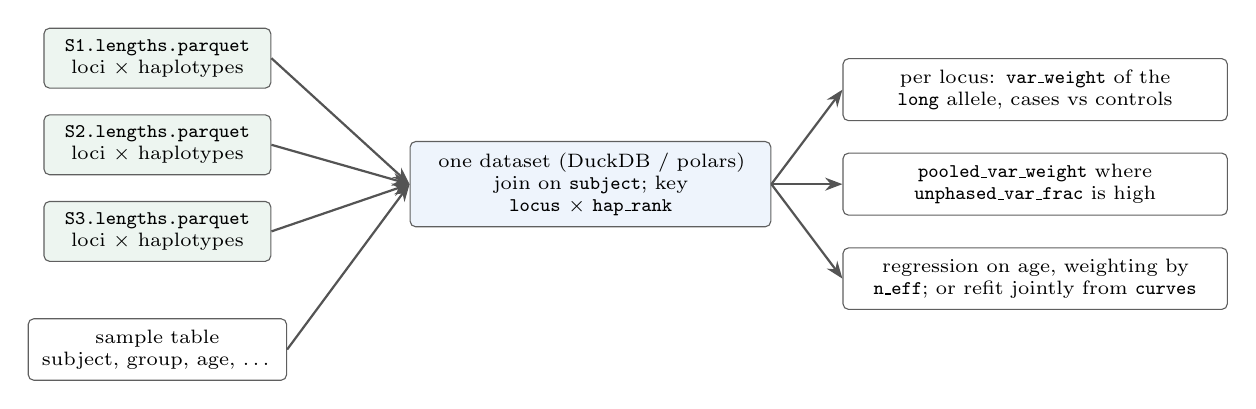
\begin{tikzpicture}[x=1mm,y=1mm]
\foreach \i/\n in {0/S1,1/S2,2/S3} {
  \node[box,fill=ok!8,text width=2.6cm,font=\scriptsize] (p\i) at (15,28-11*\i) {\texttt{\n.lengths.parquet}\\ loci $\times$ haplotypes};}
\node[box,text width=3.0cm,font=\scriptsize] (smp) at (15,-9) {sample table\\ subject, group, age, \dots};
\node[box,fill=hone!8,text width=4.3cm,font=\scriptsize] (db) at (70,12) {one dataset (DuckDB / polars)\\
join on \texttt{subject}; key \texttt{locus} $\times$ \texttt{hap\_rank}};
\foreach \i in {0,1,2} {\draw[arr] (p\i.east) -- (db.west);}
\draw[arr] (smp.east) -- (db.west);
\node[box,text width=4.6cm,font=\scriptsize,anchor=west] (a1) at (102,24) {per locus: \texttt{var\_weight} of the
\texttt{long} allele, cases vs controls};
\node[box,text width=4.6cm,font=\scriptsize,anchor=west] (a2) at (102,12) {\texttt{pooled\_var\_weight} where
\texttt{unphased\_var\_frac} is high};
\node[box,text width=4.6cm,font=\scriptsize,anchor=west] (a3) at (102,0) {regression on age, weighting by
\texttt{n\_eff}; or refit jointly from \texttt{curves}};
\foreach \j in {a1,a2,a3} {\draw[arr] (db.east) -- (\j.west);}
\end{tikzpicture}
\caption{Group comparison. HiPhase's haplotype~1 means nothing across subjects, so rows are matched by
\texttt{hap\_rank}, or the pooled columns are used.}
\end{figure}

%=====================================================================
\section{Statistical choices}
\label{sec:checks}

\begin{table}[H]
\centering\small
\begin{tabularx}{\textwidth}{@{}>{\raggedright\arraybackslash}p{3.3cm} >{\raggedright\arraybackslash}p{3.6cm} L@{}}
\toprule
choice & alternative & reason\\
\midrule
learn $p(Y\mid L,x)$ & learn $p(L\mid Y)$ & a posterior bakes in the training prior over lengths; a likelihood transfers\\
softmax over $\Delta$ bins & parametric noise head & any error shape, learned from many stable reads\\
mixture loss over alleles & hard-assign reads & heterozygous loci and unphased reads used without guessing\\
measure $Y$ between flank anchors & CIGAR inside repeat & indel placement inside repeats is arbitrary\\
soft haplotypes, $w$ from hets only & hard phasing; fit $w$ freely & free $w$ is circular: reads would go where they look least unstable\\
$\rho$ for unphased reads & 50/50 & the flank rule favours the shorter allele; fitting $\rho$ absorbs it\\
cap $w$ at $1-\epsilon$ & $w=1$ & one misphased read would become an outlier on the wrong haplotype\\
point mass + $g$ & one distribution & interpretable stable fraction $\pi$; M0 nested at $\pi=1$\\
skew-normal $g$ (default) & nonparametric $g$ & stable at modest depth; few numbers; nonparametric as a shape check\\
exclusion zone $\Delta_g$ & none & otherwise $g$ collapses on $L_0$ and absorbs $\pm1$\,bp noise\\
outlier starts, uniform EM floor & local starts only & a single expanded read must be reachable\\
selection $s(L)$ & ignore & long molecules are under-sampled by the flank rule\\
no p-values; $d_{\ell\ell}$ and baselines & bootstrap LRT & the target is estimation; stable samples give the floor\\
\bottomrule
\end{tabularx}
\caption{Choices, what they replace, and why.}
\end{table}

\paragraph{Checks on simulated loci} (\texttt{tests/test\_tandemo.py}).
\begin{itemize}
\item A haplotype with 30\% of molecules expanded is recovered at 0.23--0.41 across seeds, for both shapes. The
stable haplotype stays at 0--0.06.
\item One or two expanded reads among 40 per haplotype (+30 or +240\,bp, phased or not) are captured with a
HiFi-like noise model: $1-\pi=1/41$ or $2/42$, \texttt{n\_support} = 1 or 2, log-likelihood gain 8--20. Stable
loci give exactly 0.
\item With all reads unphased, the two haplotypes are separated by length and $\rho\approx0.5$.
\end{itemize}

\paragraph{The stable floor.} A maximum-likelihood weight at a boundary is biased upward. With a noise model whose
tails are too heavy, stable loci show $1-\pi\approx0.03$ on average at 40 reads per haplotype. Whether one or two
deviant reads count as instability is decided by Network~1's tails: a sharp, well-calibrated noise model makes
them decisive. Artefact reads (paralogs, chimeras) also produce outliers. Run Stage~2 on held-out stable samples
and read instability as an excess over that baseline at matched depth and locus class.

\begin{figure}[H]
\centering
\begin{tikzpicture}
\begin{axis}[name=a,width=0.46\textwidth,height=4.4cm,xlabel={expanded reads among 40},ylabel={$1-\pi_1$},
  legend style={font=\scriptsize,at={(0.03,0.97)},anchor=north west,draw=none},tick label style={font=\scriptsize},
  label style={font=\small},xtick={0,1,2,3,5,8}]
\addplot[hone,thick,mark=*] table[x=k,y=var_weight,col sep=comma] {figs/data/detect_sharp.csv};
\addlegendentry{sharp noise model}
\addplot[nul,thick,mark=square*,dashed] table[x=k,y=var_weight,col sep=comma] {figs/data/detect_heavy.csv};
\addlegendentry{heavy-tailed noise model}
\addplot[ink!40,domain=0:8] {x/40};
\end{axis}
\begin{axis}[at={(a.east)},anchor=west,xshift=14mm,width=0.46\textwidth,height=4.4cm,xlabel={expanded reads among 40},
  ylabel={log-likelihood gain $d_{\ell\ell}$},tick label style={font=\scriptsize},label style={font=\small},xtick={0,1,2,3,5,8}]
\addplot[hone,thick,mark=*] table[x=k,y=d_ll,col sep=comma] {figs/data/detect_sharp.csv};
\addplot[nul,thick,mark=square*,dashed] table[x=k,y=d_ll,col sep=comma] {figs/data/detect_heavy.csv};
\end{axis}
\end{tikzpicture}
\caption{$k$ reads expanded by 6--15 units among 40 phased reads of haplotype~1, median of 8 simulations. Left:
the fitted variable weight tracks $k/40$ (grey line) under both noise models, so Stage~2 does not regularise single
reads away. Right: the \emph{evidence} for them depends on Network~1's tails. With a sharp model one read gains
$\approx11$ log units and a stable locus gains 0. With heavy tails, one read gains about 6, and a stable locus already
gains about 2.}
\end{figure}

%=====================================================================
\section{Deferred}
\label{sec:later}
\begin{itemize}
\item \textbf{Truncated reads} (one good flank): a lower bound $L\geq c$, through a survival term in Network~1. They
see expansions longer than reads can span.
\item \textbf{Inside the repeat}: indel features, the motif-phase impurity spectrum, and unit decomposition by
wrap-around alignment, as extra features or priors.
\item \textbf{Allele-specific noise}: two curves per uncertain read, $\ell_i(L\mid x_1)$ and $\ell_i(L\mid x_2)$.
\item \textbf{Uncertainty intervals} for $\pi$ and $g$ (profile likelihood or bootstrap over subjects), and a group-level
model on the stored curves.
\end{itemize}

%=====================================================================
\section{Usage}
\begin{verbatim}
# 1. per sample, after minimap2 (somatic_sv/scripts/align_hifi.sh), HiPhase and TRGT
tandemo extract --bam s.bam --reference ref.fa --catalog trgt.bed.gz \
    --phased-vcf s.hiphase.vcf.gz --trgt-vcf s.trgt.phased.vcf.gz --out ex/s --threads 32

# 2. once, on stable sample(s)
tandemo train --input ex/stable1 ex/stable2 --out net1.pt          # PyTorch
tandemo train --input ex/stable1 --out noise.npz --empirical       # numpy baseline

# 3. per subject
tandemo fit --input ex/s --model net1.pt --out fit/s --threads 32 \
    [--shape nonparametric] [--write-curves]
\end{verbatim}

\end{document}
